%!TEX root = skripsi.tex
%-----------------------------------------------------------------------------%
\chapter{\babEmpat} \label{implementasi}
%-----------------------------------------------------------------------------%
Bab ini akan menjelaskan perihal implementasi dari rancangan yang sudah dibuat pada bab sebelumnya, mulai dari pembangunan \textit{sense tagged corpus} bahasa Inggris sampai dengan evaluasi.

\section{Pembangunan \textit{Sense Tagged Corpus} Bahasa Inggris}
Proses pertama yang dilakukan adalah memisahkan kalimat bahasa Inggris dan bahasa Indonesia dari korpus identik menjadi dua buah \textit{file} paralel untuk dapat diproses pada tahap-tahap berikutnya. Korpus yang dihasilkan setelah proses ini adalah dua buah korpus (korpus bahasa Indonesia, dan korpus bahasa Inggris) dimana masing-masing baris merupakan kalimat yang saling berpasangan.

\textit{Sense Tagged Corpus} dibangun dengan menggunakan bantuan IMS untuk memberikan tag pada korpus bahasa Inggris. \textit{Pre-processing} dilakukan terlebih dahulu terhadap korpus bahasa Inggris seperti menghilangkan tanda baca dan mengubah semua token menjadi huruf kecil. Proses \textit{tagging} dilakukan dengan menjalankan perintah:

\begin{lstlisting}[language=bash, caption={\textit{Tagging} korpus bahasa Inggris dengan IMS}, label={IMS}]
./testPlain.bash <model> <file_input> <file_output> <file_index_sense>
\end{lstlisting}

model yang digunakan IMS pada penelitian ini adalah model yang tersedia pada \textit{website software NUS} berdasarkan versi Wordnet 3.0. Model yang digunakan tersebut meliputi hasil \textit{training} kata-kata dalam bahasa Inggris yang sudah dibangun pada \textit{sense tagged corpus} bahasa Inggris \citep{taghipour2015one}. Proses yang dilakukan IMS dalam melakukan \textit{tagging sense} adalah dengan mengiterasikan melakukan \textit{sentence splitter}, \textit{tokenizing}, \textit{POS Tagging}, dan \textit{lemmatizing}. Setelah proses itu dilakukan, ekstraksi fitur dilakukan sebelum hasilnya masuk ke dalam \textit{classifier} berdasarkan model kata yang sudah ada. 


Hasil \textit{output} dari \textit{tool} tersebut adalah korpus dengan kata-kata sudah ditag dengan makna kata yang mungkin(dalam bentuk \textit{sense key}). Makna kata yang diambil untuk kata tersebut merupakan \textit{sense key} dengan nilai kemungkinan terbesar. \textit{Sense key} merupakan \textit{identifier} unik yang menyimpan arti dari suatu kata pada Wordnet Princeton dengan format "lemma\_suatu\_kata\%key". Untuk mempermudah pemakaian \textit{sense tagged corpus} ini pada proses selanjutnya, dilakukan \textit{post-processing} untuk mengubah hasil keluaran ke dalam format berikut.\\

\noindent\fbox{%
	\parbox{\textwidth}{%
		<sentence>kata-1||sensekey-1 kata-2||sensekey-2 ...</sentence>\\
		<sentence>kata-n||sensekey-n kata-m||sensekey-m ...</sentence>\\
		...	
	}%
}\\

Contoh dari kalimat yang sudah diberikan \textit{tag} sampai keluar dari \textit{post-processing} adalah:\\

\noindent\fbox{%
	\parbox{\textwidth}{%
		<sentence>years||year\%1:28:01:: animals||animal\%1:03:00:: have||have\%2:40:04:: caused||cause\%2:36:00:: havoc||havoc\%1:04:00::</sentence>
	}%
}\\

Pada contoh tersebut, kata years memiliki \textit{sense key} berupa "year\%1:28:01::", dimana berdasarkan Wordnet mempunyai arti sebagai '\textit{a period of time containing 365 (or 366) days}'. Tidak semua kata dalam korpus bahasa Inggris ditag oleh IMS, kata-kata sapaan seperti "I", "you", "a" , "the", dan beberapa kata lainnya tidak diberikan \textit{sense key}.  



\section{\textit{Word Alignment}}

Proses awal yang diperlukan untuk \textit{alignment} adalah memberikan kedua korpus (Indonesia dan Inggris) ke dalam input Giza++. Setelah menghasilkan \textit{file} hasil \textit{alignment}, dilakukan post-processing untuk menghasilkan kamus yang nantinya dapat digunakan untuk melakukan validasi pasangan kata pada proses \textit{sense transfering}.

\subsection{Pemrosesan \textit{Word Alignment}}
Proses \textit{word alignment} menggunakan dua buah \textit{file} yaitu korpus berbahasa Indonesia dan Inggris yang sudah dipisah dari \textit{pre-processing}. Perintah berikut digunakan untuk melakukan \textit{word alignment} dengan Giza pada penelitian ini:

\begin{lstlisting}[language=bash,caption={\textit{Word  alignment} dengan Giza++}, label={word-alignment}]
./plain2snt.out [source_language] [target_language]

./snt2cooc.out [source_language_vcb_file] [target_language_vcb_file] [snt_file] > [coocurrence_file]


./GIZA++ -S [source_language_vcb] -T [target_language_vcb] -C [snt_file] -CoocurrenceFile [cooc_file]
\end{lstlisting}

\textit{Command} tersebut dilakukan pada direktori \textit{tool} Giza++. Proses pertama akan menghasilkan tiga buuah \textit{file} yaitu dua buah \textit{file vocabulary} yang berisi nomor indeks dengan kata (bahasa asal, dan bahasa tujuan), dan satu buah \textit{file} snt yang berisi \textit{alignment} dari kalimat. Proses snt2cooc akan menghasilkan \textit{cooccurence file} yang merupakan pasangan-pasangan kalimat untuk dapat diproses Giza.

Giza mengeluarkan beberapa \textit{file} hasil dari proses tersebut. \textit{Output} yang akan digunakan diantaranya adalah \textit{file} bernama A3.final yang merupakan pasangan kalimat dengan kata-kata yang sudah dipasangkan sesuai dengan prediksi terbaik hasil pemrosesan Giza.

\subsection{Post-Processing}
Setelah mendapatkan \textit{file} A3 dari Giza, dilakukan \textit{post-processing} untuk menghasilkan \textit{file} yang dengan mudah dapat diproses untuk melakukan \textit{sense transfering}. Berikut ini merupakan salah satu contoh pasangan kalimat pada \textit{file} A3 keluaran Giza.

\begin{lstlisting}[backgroundcolor = \color{white}]
# Sentence pair (47183) source length 9 target length 9 alignment score : 6.85298e-13
Undang-Undang No 14 tahun 2008 tentang Kebebasan Memperoleh Informasi 
NULL ({ }) Law ({ 1 }) No ({ 2 }) 14 ({ 3 }) of ({ }) 2008 ({ 4 5 }) on ({ 6 }) Freedom ({ 7 8 }) of ({ }) Information ({ 9 })
\end{lstlisting}

Pembacaan pasangan kata berdasarkan hasil keluaran dilakukan dengan indeks nomor kata yang berada pada dalam kurung kata di bahasa Inggris. Karena pemisah token \textit{by default} adalah spasi, maka kata "Undang-Undang" adalah kata dengan indeks nomor 1, kata "No" diberikan indeks nomor 2, dan berlaku hal yang sama sampai kata "Informasi". Pada kata bahasa inggris, "Law" dipasangkan dengan indeks satu yang mana adalah "Undang-Undang", kata "No" dipasangkan dengan indeks dua yang mana adalah "No", dan selanjutnya sampai kata \textit{Information}. 

Terdapat dua buah \textit{post-processing} yang dilakukan dengan tujuan masing-masing untuk:

\begin{enumerate}
	\item Penyimpan pasangan kata-kata yang bersesuaian untuk sistem WSD.
	\item Sebagai \textit{resource} untuk proses \textit{enhancement word alignment}.
\end{enumerate}


Untuk keperluan nomor satu, bentuk \textit{output} diproses menjadi bentuk lain dengan format:\\

\noindent\fbox{%
	\parbox{\textwidth}{%
		<pair>kata\_en\_1||kata\_id\_1 kata\_id\_2</pair>\#\#<pair>kata\_en\_2||kata\_id\_3\\</pair>...</pair>
	}%
}\\


Contoh dari hasil \textit{post-processing} pada pasangan kalimat sebelumnya adalah:

\begin{lstlisting}[backgroundcolor = \color{white}]
<pair>law||undang-undang</pair>##<pair>no||no</pair>##<pair>14||14</pair>##<pair>2008||tahun 2008</pair>##<pair>on||tentang</pair>##<pair>freedom||kebebasan memperoleh</pair>##<pair>information||informasi</pair>
\end{lstlisting}

Hasil ini kemudian disimpan sebagai sebuah \textit{file} sendiri yang akan digunakan kembali pada proses selanjutnya. Sementara itu, keperluan nomor dua difokuskan untuk membuat \textit{dictionary} yang akan ditingkatkan kualitasnya pada tahap berikutnya. Untuk menghasilkan \textit{file} yang dibutuhkan pada nomor kedua, dilakukan pengumpulan pasangan kata bahasa Indonesia dengan bahasa Inggris. Bila misalkan pada kalimat ke-n terdapat kata "undang-undang" yang dipasangkan dengan "law", dan pasangan kata "undang-undang" dengan "regulation" pada kalimat lain (kalimat ke-m, dimana m != n). Berdasarkan kedua kalimat tersebut, maka kata "undang-undang" akan berpasangan dengan dua kata yaitu "law", dan "regulation".

\section{Peningkatan Kualitas \textit{Alignment}}

Hasil dari \textit{alignment} kata yang dilakukan Giza masih menghasilkan pasangan-pasangan kata yang tidak tepat. Untuk mengurangi jumlah pasangan kata yang salah tersebut, dilakukan \textit{enhancement} terhadap hasil pasangan kata dari Giza. Terdapat dua macam peningkatan kualitas \textit{alignment} yang digunakan pada penelitian ini, yaitu \textit{crawling based} dan \textit{bi-directional based}.

\subsection{Pendekatan \textit{Crawling}}

Konsep \textit{crawling} pada penelitian ini mengacu pada kebutuhan untuk \textit{filtering} hasil pasangan kata yang salah berdasarkan kamus Indonesia-Inggris. Karena keterbatasan \textit{resource digital} kamus tersebut, maka dibutuhkan pendekatan \textit{crawling} dari \textit{online dictionary} untuk mendapatkan pasangan kata yang benar. Salah satu \textit{online dictionary} yang dapat diakses dan memiliki hasil terjemahan yang cukup baik adalah \textit{website} sederet.com. \textit{Crawling} dilakukan dengan memeriksa setiap pasangan bahasa Inggris dari kata Indonesia hasil Giza, apakah pasangan kata tersebut berada pada hasil penerjemahan yang sesuai. Ilustrasi dari proses ini dapat dimodelkan dalam contoh berikut:

\begin{enumerate}
	\item Kata "halaman" memiliki pasangan bahasa Inggris hasil Giza yaitu  "\textit{courtyard}", \textit{"yard"}, \textit{"page"}, dan "\textit{lawn}".
	\item Gunakan \textit{crawler} untuk menerima hasil terjemahan dari kata "halaman" dalam bahasa Inggris
	\item \textit{Crawler} mendapatkan hasil kata "\textit{page}", dan "\textit{courtyard}".
	\item Berdasarkan kedua hasil tersebut, maka pasangan kata "halaman" yang dianggap benar adalah irisan dari kedua \textit{set} tersebut yaitu "\textit{page}" dan "\textit{courtyard}"
\end{enumerate}

\subsection{Pendekatan \textit{Bi-directional}}

Metode lain yang digunakan untuk meningkatkan kualitas \textit{aligment} yaitu dengan memanfaatkan \textit{bi-directional alignment}. Proses yang dilakukan adalah melakukan validasi terhadap kata-kata yang berpasangan  dari kedua korpus. \textit{Source code} dari proses \textit{enhancement bi-directional} ini dapat dilihat pada kode berikut.

\begin{lstlisting}[language=Python, caption={Word Alignment Enhancement}, label={word-alignment-enhancement}]

dict_id = {}
dict_en = {}


# this section is for filtering which english word that has corresponding indo translation (bidirectional) from Giza output
for indo_word in dict_id.keys():
	for en_word in dict_id[indo_word].keys():
		if en_word != dict_en:
		# filtering so no same translation is entered, answer -> answer, jawaban -> jawaban
			if en_word in dict_en and indo_word in dict_en[en_word] and en_word not in stop:
				if indo_word not in final_dictionary:
					final_dictionary[indo_word] = { en_word: dict_en[word_en][word_id] }
				else:
					if en_word not in final_dictionary[indo_word]:
						final_dictionary[indo_word][en_word] = dict_en[word_en][word_id]
\end{lstlisting}

Pertama, setiap kata dalam bahasa Indonesia dikumpulkan terlebih dahulu dengan setiap pasangan kata bahasa Inggrisnya (satu kata bisa memiliki lebih dari satu pasangan) ke dalam variabel dict\_id. Proses selanjutnya adalah melakukan pengumpulan yang serupa terhadap kata dalam bahasa Inggris dengan pasangan kata dalam bahasa Indonesianya (pada variabel dict\_en). Berbagai kata dalam bahasa Indonesia beserta pasangannya disimpan sebagai "kamus-1 (dict\_id)". Kata dalam bahasa Inggris, beserta pasangan kata Indonesianya disimpan sebagai "kamus-2"(dict\_en). Variabel stop berisi \textit{list} of stopwords Bahasa Inggris dari \textit{library} NLTK. Proses validasi kebenaran dari pasangan kata dilakukan dengan cara:

\begin{enumerate}
	\item Untuk setiap kata di bahasa Indonesia dalam "kamus-1" semisal kata "kali".
	\item Lakukan pengecekan terhadap setiap pasangan kata di bahasa Inggris pada "kamus-1" dari kata "kali", misalkan pasangan kata bahasa inggrisnya adalah "time", "river", dan "fire".
	\item Jika pada "kamus-2" kata "time" dipasangkan dengan "kali", dan "waktu" maka kata "time" merupakan pasangan yang dianggap benar (karena kata "time" berpasangan dengan "kali"). Pada kasus kata "fire", bila pasangan bahasa Indonesianya adalah "api" dan "tungku", maka kata "fire" dianggap bukan pasangan yang tepat dengan "kali" karena tidak terdapat pasangan "fire -> kali".
\end{enumerate} 


\section{\textit{Sense Transfering}}
Hasil dari proses peningkatan kualitas \textit{alignment} adalah sebuah "kamus" bahasa yang akan digunakan sebagai referensi untuk memindahkan makna kata dari bahasa Inggris ke kata yang benar pada bahasa Indonesia. Proses ini dilakukan dengan tahap-tahap sebagai berikut:

\begin{enumerate}
	\item Iterasi untuk setiap kata dalam bahasa Indonesia pada kamus
	\item Iterasi pada setiap pasangan kalimat
	\item Periksa apakah "\textit{pair}" kata bahasa Indonesia tersebut terdapat di dalam kamus
	\item Jika "pair" tersebut benar berada dalam kamus, maka pindahkan makna kata dari \textit{english word} yang bersesuaian.
\end{enumerate}

Ilustrasi dari proses tersebut pada kata "halaman" secara garis besar dapat dilihat pada gambar 


\begin{figure}
	\centering
	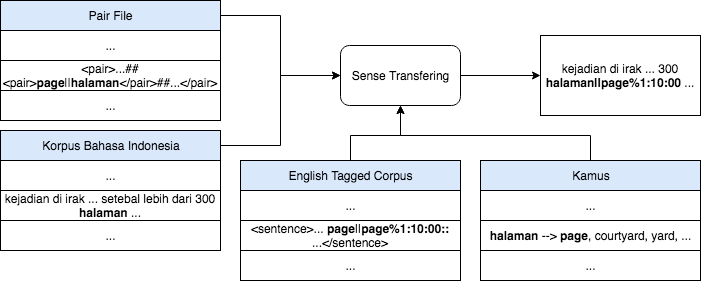
\includegraphics[width=1\linewidth]{adit_pics/sense-transfering}
	\caption{Ilustrasi \textit{sense transfering}}
	\label{fig:ilustrasi-sense-transfering}
\end{figure}

Proses yang terjadi pada ilustrasi di atas adalah:

\begin{enumerate}
	\item Jika misalkan kata "halaman" pada kamus memiliki pasangan kata "page" dan "courtyard".
	\item Pada sebuah kalimat "... 300 halaman ..." dimana "\textit{pair}" pada kalimat tersebut diantaranya adalah
	\begin{lstlisting}[backgroundcolor = \color{white}]
	..<pair>second||kedua</pair>##<pair>page||halaman</pair>..
	\end{lstlisting}
	\item Pasangan kata yang didapat dari "halaman" dari \textit{pair} tersebut adalah "page". Berdasarkan hasil tersebut kata "page" kemudian diperiksa pada kamus yang ada.
	\item Karena kata "page" merupakan salah satu terjemahan untuk kata "halaman", maka pindahkan makna "page" dari \textit{sense tagged corpus} kalimat tersebut ke kata "halaman" pada kalimat Indonesia dengan indeks yang sama. Hal tersebut dapat dicontohkan pada pemindahan makna "page\%1:10:00::" dari contoh \textit{sense tagged corpus} berikut.
	\begin{lstlisting}[backgroundcolor = \color{white}]
	<sentence>... page||page%1:10:00:: ...</sentence>
	\end{lstlisting}
	\textit{Sense key} "page\%1:10:00::" tersebut kemudian dipindahkan ke kata "halaman" pada kata "halaman" di kalimat bahasa Indonesia yang bersesuaian.
	\item Dalam proses pemindahan makna tersebut, akan dilakukan pemeriksaan apakah untuk kata yang sama, terdapat makna kata yang serupa dari hasil transfer kalimat lain.
	\item Jika "kemiripan" makna kata yang akan dipindahkan melebihi threshold (0.5), makan akan digunakan \textit{sense key} yang lama karena kedua \textit{sense key} dianggap mempunyai makna yang sama. Penghitungan seberapa dekat "makna" dari kedua \textit{sense key} tersebut dilakukan dengan bantuan \textit{method} path\_similarity dari \textit{tool} NLTK dengan korpus wordnet.
\end{enumerate}

Setelah didapatkan setiap kata beserta makna hasil \textit{transfernya}, semua kata tersebut disusun ke dalam bentuk JSON dengan bentuk \textit{array of} kalimat yang isinya adalah \textit{array of words}. Setiap \textit{instance} dari \textit{word} tersebut menyimpan kata, POS Tag, dan \textit{sense key} hasil \textit{sense transfering} jika ada.
%-----------------------------------------------------------------------------%
\section{WSD Bahasa Indonesia}
Sistem WSD dibangun dengan menggunakan \textit{supervised learning}. Pada sistem ini terdapat tiga buah bagian utama yaitu pemilihan fitur serta \textit{classifier}, ekstraksi fitur, dan evaluasi hasil \textit{classifier}. Proses yang pertama kali dilakukan oleh sistem adalah membaca korpus dan memilih \textit{target word}, mendapatkan \textit{sense key} dari kata tersebut untuk dijadikan sebagai \textit{class} dari klasifikasi. Pada sistem WSD yang dibuat, kata-kata yang terdapat pada \textit{list of stopwords} dihilangkan dari kalimat-kalimat pada data.

\subsection{Pemilihan Fitur dan \textit{Classifier}}
Terdapat tiga buah fitur pada penelitian ini yang terdiri dari:

\begin{enumerate}
	\item Fitur \textit{bag of words}
	\item Fitur \textit{POS tagging}
	\item Vektor dari hasil \textit{word embedding}
\end{enumerate}

\textit{Classifier} yang digunakan pada penelitian ini adalah SVM dari Scikit \citep{scikit-learn} dengan parameter \textit{default} berupa kernel linear dan C=1. Penggunaan SVM pada penelitian ini mengikuti \textit{classifier} yang digunakan pada IMS \cite{zhong2010makes} untuk melihat performa yang dihasilkan pada sistem WSD Bahasa Indonesia yang dibuat.

\subsection{Ekstraksi Fitur}
Proses yang dilakukan dalam pengambilan kata konteks untuk fitur \textit{bag of words} dilakukan dengan tahap-tahap berikut.

\begin{lstlisting}[language=python,caption={Fitur Bag of Words}, label={fitur-bag-of-words}]

bag_of_words []

for each sentence
split sentence by whitespace into words
for each word
if word == target word
for x in [-2,-1,1,2]
if word(x) exist and word(x) not in bag_of_words
add word(x) into bag_of_words

return bag_of_words

\end{lstlisting}

Pada \textit{source code} tersebut, fitur \textit{bag of words} diinisiasi dengan \textit{list} kosong. Proses selanjutnya adalah dengan mengiterasi setiap kata dalam setiap kalimat, jika kata tersebut merupakan \textit{target word} yang dicari, ambil kata dengan indeks -2, -1, 1, dan 2 dari kata \textit{target word} sekarang (jika ada). Hasil dari proses tersebut adalah \textit{list} yang berisi kata-kata yang pernah muncul sebagai tetangga dari \textit{target word}. Kumpulan kata-kata tersebut kemudian digunakan untuk mengubah suatu kalimat yang mengandung \textit{target word} menjadi vektor yang merepresentasikan keberadaan kata-kata pada \textit{list bag of words} tersebut.

Fitur POS Tagging menggunakan \textit{tool} dari Stanford bernama "A Part-Of-Speech Tagger" yang dilatih dengan menggunakan model untuk bahasa Indonesia \citep{dinakaramani2014designing}. Proses \textit{tagging} ini dilakukan sebelum memasuki sistem WSD terhadap keseluruhan kalimat dalam korpus identik yang berisi bahasa Indonesia saja. Terdapat \textit{pre-processing} awal pada korpus bahasa Indonesia tersebut untuk menghilangkan beberapa tanda baca seperti titik, koma, tanda tanya, tanda seru, dan beberapa tanda baca lainnya. Setelah proses tersebut, diberikan tanda baca berupa titik pada akhir kalimat sebagai indikator akhir sebagai kebutuhan dari kompabilitas \textit{tool} (tidak semua kalimat pada korpus memiliki tanda baca akhir kalimat). Perintah yang dilakukan untuk melakukan \textit{POS Tagging} tersebut adalah:

\begin{lstlisting}[language=bash,caption={Stanford POS Tagger}, label={stanford-pos-tagger}]

java -mx300m -cp 'stanford-postagger.jar:lib/*' edu.stanford.nlp.tagger.maxent.MaxentTagger -model <model_bahasa_indonesia> -textFile <korpus_bahasa_indonesia>

\end{lstlisting}

Hasil dari proses tersebut merupakan korpus dengan setiap kata yang sudah memiliki POS Tag dengan format:

\begin{lstlisting}[backgroundcolor = \color{white}]
<kata_1>_<postag_1> <kata_2>_<postag_2> ... <kata_n>_<postag_n>
<kata_x> <postag_x> <kata_y>_<postag_y> ... <kata_z>_<postag_z>
...
\end{lstlisting}

Proses dalam melakukan eksetraksi fitur POS Tag tersebut dapat dilihat pada \ref{fitur-postag} berikut.

\begin{lstlisting}[language=python,caption={Ekstraksi Fitur POS Tag}, label={fitur-postag}]

pos_tag_features = [[],[],[]]

foreach sentence in pos_tagged_sentences:
	foreach word_with_postag in sentence:
		word, postag = split_postag(word_with_postag)
		if word == target_word:
			if word_before(word,-1) exist:
				pos_tag_features[0].append(postag(word,-1))
			pos_tag_features[1].append(postag)
			if word_after(word,1) exist:
				pos_tag_features[2].append(postag(word,1))

\end{lstlisting}

Pada proses ekstraksi fitur POS Tag, dilakukan iterasi untuk setiap kata pada setiap kalimat. Jika \textit{target word} telah ditemukan, ambil POS Tag dari kata sebelum \textit{target word}, \textit{target} word, dan sesudah \textit{target word}. pos\_tag\_features[0] merepresentasikan POS Tag yang muncul pada sebelum \textit{target word}, pos\_tag\_features[1] untuk POS Tag \textit{target word}, dan pos\_tag\_features[2] untuk POS Tag kata sesudah \textit{target word}. Setelah POS Tag masing-masing posisi dikumpulkan, vektor representasi fitur akhir akan bernilai satu jika POS Tag muncul pada kalimat dan nol jika POS Tag tidak muncul. 

Fitur ketiga adalah penggunaan vektor dari model \textit{word embedding}. Ekstraksi fitur ini dilakukan dengan proses \ref{ekstraksi-we-feature}.

\begin{lstlisting}[language = python, caption={Ekstraksi fitur \textit{word embedding}}, label={ekstraksi-we-feature}]

model = Word2Vec.load(word_embedding_model)

length_we_feature = len(model['yang'])

max_length = max(length(sentences))

foreach sentence in sentences_containing_target_words:
	arr = []
	words = get_words(sentence)
		for x in range(max_length):
			if x in range of len(words):
				if words[x] in model:
					arr = arr + model[words[x]]
				else:
					arr = arr + array_of_zero(length_we_feature)
			else:
				arr = arr + array_of_zero(length_we_feature)
\end{lstlisting}

Pada proses tersebut, \textit{length\_we\_feature} diisi dengan jumlah kata terbanyak pada kumpulan kalimat. Untuk setiap kalimat, setiap kata di dalamnya akan diperiksa terlebih dahulu apakah terdapat vektor kata tersebut pada model. Jika vektor kata tersebut ada pada model \textit{word embedding} yang digunakan, konkatenasi vektor dengan arr yang merepresentasikan fitur pada kalimat tersebut. Namun demikian, jika kata tersebut tidak terdapat pada model ataupun indeks kata sudah melebihi jumlah kata pada kalimat, konkatenasi arr dengan \textit{array} yang berisi angka nol sebanyak panjang dari vektor \textit{word embedding}.

Fitur terakhir yang dicoba adalah gabungan dari fitur \textit{bag of words} dengan \textit{POS Tag}. Implementasi yang digunakan sama dengan ekstraksi fitur \textit{bag of words} dan POS Tag, yang kemudian kedua buah vektor dikonkatenasi menjadi satu buah vektor gabungan.

\section{Evaluasi dan Anotasi}

Proses evaluasi meliputi \textit{pre-processing}, anotasi data, dan evaluasi. Hasil dari evaluasi ini ditujukan untuk memberikan informasi seberapa baik performa dari \textit{alignment} yang dilakukan oleh \textit{tool} Giza. Terdapat beberapa proses dalam mempersiapkan data untuk evaluasi oleh anotator.
\begin{enumerate}
	\item Pertama, pada setiap kata dalam bahasa Indonesia diberikan sebuah tanda indeks berupa angka untuk mempermudah proses evaluasi anotator nantinya. Pada proses tersebut, kalimat "Aku ingin makan" sebagai perumpamaan, diubah menjadi "Aku(1) ingin(2) makan(3)". Angka tersebut diperuntukan untuk mempercepat dan mempermudah kerja anotator nanti untuk melihat pasangan kata dari kalimat bahasa Inggris.
	\item Kedua, kosongkan nomor indeks hasil \textit{alignment} Giza pada kalimat bahasa Inggris. Perumpamaan pada kalimat "NULL (\{  \}) i (\{ 1 \}) want (\{ 2 \}) to (\{  \}) eat (\{ 3 \})" akan berubah menjadi  "NULL (\{  \}) i (\{  \}) want (\{   \}) to (\{  \}) eat (\{  \})" yang nantinya akan diisi secara manual oleh anotator.
\end{enumerate}

\subsection{Anotasi}
Setelah diberikan pasangan kalimat untuk dianotasi, anotator melakukan anotasi sesuai dengan panduan yang diberikan. Hasil dari anotasi tersebut kemudian dikumpulkan kembali untuk dievaluasi.

\subsection{Evaluasi \textit{Word Alignment}}
Evaluasi perhitungan \textit{precision}, \textit{recall}, f-score, dan \textit{agreement} merupakan penyesuaian dari rumus pada \citep{mihalcea2003evaluation}. Perhitungan dilakukan secara otomatis dengan program yang dibuat dengan algoritma berikut.

\begin{lstlisting}[language=Python, caption={Word Alignment Evaluation}, label={word-alignment-evaluation}]

def evaluate_bracket(list_giza, list_anotator):
# evaluate per character
numbers_anotator = len(list_anotator)
numbers_giza = len(list_giza)
match = 0
if numbers_giza < numbers_anotator:
# iterate through the numbers giza
for n in list_giza:
if n in list_anotator:
match += 1
else:
# iterate through the numbers anotator
for n in list_anotator:
if n in list_giza:
match += 1
return (numbers_anotator, numbers_giza, match)

# given sentence which already been alignned from the first anotator (an1), second anotator(an2), and giza(giza)
matches, total_giza, total_anotator, total_giza_1, total_anotator_1 = 0, 0, 0, 0, 0
precision, recall = [[],[]], [[],[]]

for each sentence in sentences:
for each token in sentence:
(numbers_anotator, numbers_giza, match) = evaluate_bracket(an1(token), giza(token))
(numbers_anotator_1, numbers_giza_1, match_1) = evaluate_brakcet(an2(token), giza(token))
agreement = count_agreement(an1(token), an2(token))
matches += match
matches_1 += match_1
total_giza += numbers_giza
total_giza_1 += numbers_giza_1
total_anotator += numbers_anotator
total_anotator_1 += numbers_anotator_1
agreement.append(agreement)
precision[0].append(matches/total_giza)
recall[0].append(matches/total_anotator)
precision[1].append(matches_1/total_giza_1)
recall[1].append(matches_1/total_anotator_1)

precision = average(precision[0])
recall = average(recall[0])
precision_1 = average(precision[1])
recall_1 = average(recall[1])
f1 = 2 * precision * recall / (precision + recall)
f2 = 2 * precision_1 * recall_1 / (precision_1 + recall_1)
agreement = average(agreement)	

\end{lstlisting}

Berdasarkan cara perhitungan evaluasi tersebut, terdapat dua buah \textit{precision} dan \textit{recall} yang mana masing-masing menunjukan indikator penilaian untuk anotator pertama dan kedua. Precision didapatkan dengan menghitung jumlah \textit{alignment} yang sama antara anotator dengan hasil giza, dibagi dengan jumlah \textit{alignment} pada Giza. Sementara itu, Recall dihitung dengan cara jumlah \textit{alignment} sama dibagi dengan jumlah \textit{alignment} pada Anotator. Nilai F-score dihitung dengan cara mengalikan 2 dengan Precision dan Recall, lalu membaginya dengan jumlah Precision dan Recall. Precision, Recall, dan F-score masing-masing kalimat kemudian dirata-rata untuk mendapatkan nilai akhir. Agreement pada kedua anotator dilihat dengan membandingkan antara jumlah kesamaan \textit{alignment} pada kedua anotator dibagi dengan jumlah \textit{alignment} anotator pertama.

\subsection{Evaluasi Sistem WSD Bahasa Indonesia}
\textit{Target word} untuk evaluasi dipilih secara manual yang memenuhi kriteria bahwa kata tersebut memiliki kata \textit{translation} lebih dari satu dengan makna masing-masing yang berbeda. Evaluasi dilakukan dengan 4-Fold \textit{cross validation} menggunakan perhitungan F1-score dari hasil klasifikasi yang dilakukan SVM terhadap \textit{target word}. Perintah pada \textit{script} yang digunakan untuk inisialisasi \textit{classifier} dapat dilihat pada potongan kode \ref{svm-command} berikut.

\begin{lstlisting}[language=python, caption={Inisialisasi SVM, baseline}, label={svm-command}]
clf = svm.SVC(kernel='linear')
bf = dummy.DummyClassifier(strategy='most_frequent')
\end{lstlisting}


\textit{Cross validation} (CV) dilakukan dengan 4-Fold CV dengan mengambil hasil akurasi (F-Score) rerata dari tiap \textit{fold}. Sebuah algoritma sederhana digunakan sebagai \textit{baseline} untuk pembanding dari sistem WSD yang dibangun. Baseline menggunakan pendekatan \textit{most frequent} sebagai cara untuk menentukan makna terbaik dari suatu kata. Baseline tersebut akan memberikan kelas makna kata pada semua \textit{target word} sesuai dengan makna kata terbanyak pada \textit{training data}.
